
\section{Method}
\label{sec:method}

\subsection{Cascade Ordering}
\label{sec:cascade}

If distributional collapse follows a predictable ordering across metrics, the earliest-responding metric can serve as a canary signal.
We formalize known metric properties (entropy as a continuous indicator of mode concentration, diversity as a threshold indicator of lexical coverage) under mode amplification~\citep{shumailov2024curse,dohmatob2024tale} (notation in Appendix~\ref{app:background}; derivations in Appendix~\ref{app:cascade_theory}).

\begin{observation}[Entropy responds before diversity]\label{thm:entropy_leads}
Under mode amplification: \textup{(a)} entropy can decrease while the $\epsilon$-effective support $S_\epsilon(p) {=} |\{i: p_i > \epsilon\}|$ (hence distinct-$n$) is unchanged; \textup{(b)} if distinct-$n$ decreases, entropy has already decreased.
\end{observation}

Intuitively, entropy responds to any redistribution of probability mass (a continuous change), whereas diversity metrics like distinct-$n$ only change when tokens are pushed entirely below the generation threshold (a discrete event).
This measurement asymmetry ensures entropy shifts before diversity under gradual mode amplification.
The margin $\gamma = \min_{i: p_i > \epsilon}(p_i - \epsilon)$ quantifies how much shift diversity absorbs silently.

\begin{observation}[Diversity lag $\geq 1$ generation]\label{prop:div_lag}
If the self-training map $\mathcal{T}$ satisfies $\alpha\|\mathcal{T}(p_t) - p_t\|_\infty < \gamma(p_t, \epsilon)$ per generation through entropy onset $t_H$, then diversity onset $t_D \geq t_H + 1$.
\end{observation}

ECE co-moves with entropy at zero lag ($\Delta\mathrm{ECE} \approx \Delta C > 0$ whenever $\Delta\bar{H} < 0$; Appendix~\ref{app:cascade_theory}), yielding a three-stage cascade $\{H, \mathrm{ECE}\} \to \mathrm{Distinct}$-$n$.
This ordering holds in 14/15 experiments at $\alpha \geq 0.30$, with entropy and ECE consistently reaching onset at generation~1 and distinct-$n$ following at generation~2 ($t_H{=}t_{\mathrm{ECE}}{=}1$, $t_D{=}2$; \S\ref{sec:regime}; Appendix~\ref{app:moment_cascade}).
The one exception, SmolLM3-3B (3/8 at $\alpha{=}1.0$; Table~\ref{tab:generalization}), shows entropy decoupling from diversity, violating the monotonic-decline assumption that underlies both Observations.
The cascade is also specific to diversity metrics: first-differencing eliminates canary$\to$perplexity associations entirely ($F{\approx}0$, $p{=}0.99$; \S\ref{sec:regime}), confirming that the temporal structure is channel-specific rather than global.

\subsection{Design Considerations}
\label{sec:pitfalls}

We use \emph{Granger precedence}, temporal predictive improvement where past values of $X$ improve prediction of $Y$ beyond $Y$'s own history, to assess whether canary metrics anticipate downstream degradation~\citep{granger1969investigating}.
This is distinct from Granger causality, which additionally implies a mechanistic causal link that bivariate tests cannot establish~\citep{shojaie2022granger}.
Even within this narrower scope, lead-lag analysis in iterative model collapse is fragile along three axes.
\emph{Method sensitivity}: five detection methods applied to identical data yield forward significance rates spanning 0\% to 92\%, with $\kappa{=}0.187$ (Figure~\ref{fig:method_comparison}).
\emph{Spurious regression}: first-differencing eliminates canary$\to$perplexity associations ($F{\approx}0$, $p{=}0.99$) while preserving canary$\to$diversity (24/24$\to$24/24)~\citep{granger1974spurious}.
\emph{Regime dependence}: the same Granger test shifts from 0/8 to 6/8 significant pairs within a 2-percentage-point interval.

\begin{figure}[t]
\centering
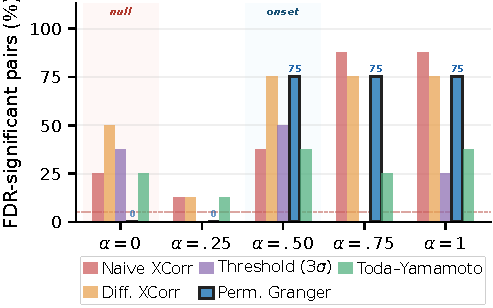
\includegraphics[width=\columnwidth]{figures/fig_method_comparison.pdf}
\caption{Method sensitivity: five methods yield dramatically different FDR-significant rates on identical data. PermG achieves the lowest null-control FPR (6.7\%, pooled across 10~seeds) with 75\% detection at $\alpha{\geq}0.50$; dashed line: 5\% nominal.}
\label{fig:method_comparison}
\end{figure}

\subsection{Method Sensitivity Analysis}
\label{sec:mmct}

These fragilities motivate a systematic comparison.
We evaluate five lead-lag detection methods (naive cross-correlation (NaiveXCorr), differenced cross-correlation (DiffXCorr), threshold onset, permutation Granger causality (PermG), and Toda--Yamamoto~\citep{toda1995statistical}) in a multi-method comparison framework~\citep{simonsohn2020specification}, calibrating each against null-control ($\alpha{=}0.0$) data.
Among these, PermG assesses whether past values of a canary metric improve prediction of a downstream metric beyond its own history~\citep{shojaie2022granger}, using 5{,}000 permutations~\citep{phipson2010permutation} on first-differenced series with Benjamini--Hochberg FDR correction ($q{=}0.05$) across 8 canary$\to$downstream pairs; the permutation null controls Type~I error by construction, and BH-FDR remains valid under positive regression dependence~\citep{benjamini2001control}.
The full multi-method consensus test (MMCT) is given in Algorithm~\ref{alg:mmct}.

\begin{algorithm}[H]
\caption{Multi-Method Consensus Test (MMCT)}
\label{alg:mmct}
\begin{algorithmic}[1]
\Require Time series pair $(X, Y)$; methods $\{m_1, \ldots, m_K\}$ ($K{=}5$); null-control data $\mathcal{N}$ (from $\alpha{=}0.0$); tolerance $\epsilon{=}0.01$
\Ensure $p$-value, consensus level $\hat{K}$
\For{each method $m_k$}
    \State Compute empirical FPR: $\widehat{\mathrm{FPR}}_k \gets$ fraction of null-control pairs where $m_k$ rejects $H_0$
    \State Compute weight: $w_k \gets 1 / \max(\widehat{\mathrm{FPR}}_k,\; \epsilon)$
    \State Apply $m_k$ to $(X, Y)$: $d_k \gets \mathbf{1}[m_k \text{ rejects } H_0]$
\EndFor
\State Weighted consensus: $W(X {\to} Y) \gets \sum_{k} w_k \, d_k \;/\; \sum_{k} w_k$
\State Build empirical null distribution of $W$ from all null-control pairs in $\mathcal{N}$
\State Compute $p$-value from empirical null: $p \gets \Pr_{\mathcal{N}}(W \geq W_{\mathrm{obs}})$
\State Consensus level: $\hat{K} \gets \sum_{k} d_k$
\State \Return $p$, $\hat{K}$
\end{algorithmic}
\end{algorithm}

\begin{figure*}[t]
\centering
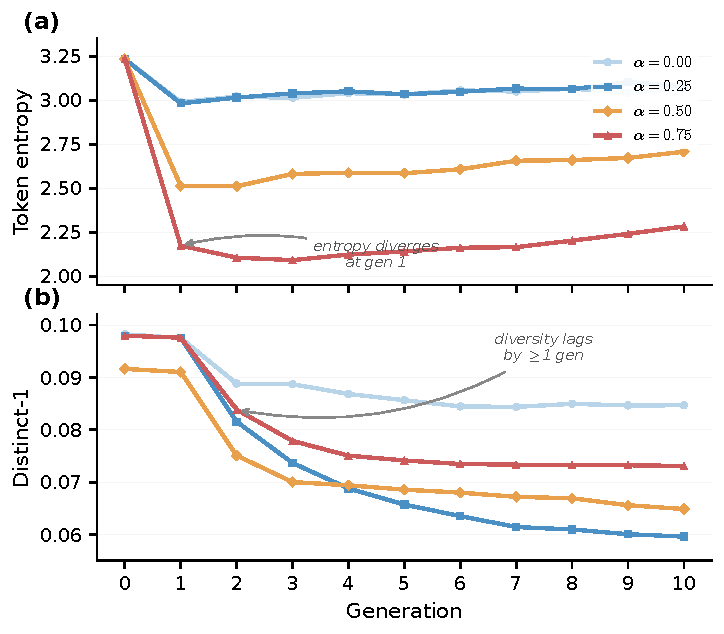
\includegraphics[width=\textwidth]{figures/metric_trajectory.pdf}
\caption{Metric trajectories at $\alpha{=}1.0$ (Pythia-410M, 4~seeds). Token entropy drops at generation~1; distinct-1 declines from generations~2--3, with a consistent one-generation canary lead (shaded: inter-seed range).}
\label{fig:metric_trajectory}
\end{figure*}

The algorithm's FPR-inverse weighting assigns each method influence proportional to its null-control reliability: NaiveXCorr (FPR${=}94.4\%$) receives weight $w{=}1.06$, while PermG (FPR${=}6.7\%$) receives $w{=}14.9$, a $14{\times}$ differential that ensures the most reliable method dominates the consensus.
Building the null distribution empirically from $\alpha{=}0.0$ data avoids parametric assumptions unreliable for short ($T{=}5$--$20$), non-stationary series.
Pooled null-control FPR across ten seeds (60 pairs) confirms a wide methodological spread: PermG 6.7\% (95\% CI $[1.8\%, 16.2\%]$), DiffXCorr 14.8\%, Threshold 24.1\%, Toda--Yamamoto 33.3\%, NaiveXCorr 94.4\% (Appendix~\ref{app:fpr_independence}).
PermG (4/60; 95\% CI $[1.8\%, 16.2\%]$) achieves the lowest FPR among all five methods, with 8/10 seeds yielding zero false positives; Shapley analysis confirms it provides the best FPR--FNR tradeoff among directional methods (Appendix~\ref{app:shapley}).
Table~\ref{tab:mmct_k_operating} reports an alternative operating mode: equal-weight $K{\geq}3$ majority voting with forward-direction filtering, where FPR is 10.0\% with 75\% TPR at $\alpha{=}1.0$ (consensus heatmap in Appendix~\ref{app:mmct}).
The weighted scheme (Algorithm~\ref{alg:mmct}) further downweights unreliable methods via FPR-inverse weighting (robust across four alternative schemes; Appendix~\ref{app:weight_robustness}); majority voting treats all methods equally and is simpler to deploy.



\subsection{Detection Boundary}
\label{sec:theory}

The steep onset described above suggests a detection boundary $\alpha_c(T)$ that decreases with longer observation.
We parametrize this boundary as a power law:
\begin{equation}
\alpha_c(T) = A \cdot T^{-\eta},
\label{eq:alpha-c}
\end{equation}
motivated by an empirical sub-linear signal model $S(\alpha) = c \cdot \alpha^\beta$ ($\beta < 1$), under which the exponent satisfies $\eta = 1/(2\beta)$:
\begin{equation}
\alpha_c(T) = A \cdot T^{-\eta},
\label{eq:alpha-c-theory}
\end{equation}
where $A = (z^* \sigma / c)^{1/\beta}$ and $z^* = \Phi^{-1}(\pi^*)$ (derivation in Appendix~\ref{app:alpha_c_proof}).
This parametrization captures the observed pattern with three free parameters fitted to 3--4 data points; the resulting $\eta$ confidence interval ($[0.64, 2.08]$) is wide enough to preclude distinguishing sub-linear from super-linear decay, but the qualitative conclusion (detection improves with longer observation) is robust regardless.

Dense $\alpha$ sampling further reveals that a smooth sigmoid fits better than a step function ($\Delta\mathrm{AIC}{=}-110$), yet the fitted onset steepness ($k{=}15.7$) exceeds smooth-model predictions by ${\sim}3{\times}$ (Appendix~\ref{app:power_sim}), suggesting the transition is sharper than standard power-analysis models would predict.
